\chapter{Background}     

\section{Introduction}
Web applications have in the last few years seen a dramatic change in both behavior and magnitude. They have grown from being a collection of simple and static Web pages into highly dynamic, and interactive applications with rich user interfaces. Previously, interactive behavior in Web sites were usually performed by Java applets and Flash applications \cite{spa} that could run inside the browser. But as JavaScript engines and Web browsers have become significantly more powerful, such behavior is increasingly being implemented exclusively with JavaScript\cite{spa}. Together with this shift towards highly interactive Web applications, the user behavior is at the same time increasingly becoming more social. Users make up the main data content of Web applications by socially interacting with each other and adding content to the pages. 

This chapter outlines recent trends in applications that can be found on the Internet; commonly named  Web 2.0\cite{web20book}. We look at the technologies that enable applications to run on the Internet, and more specifically, the software architectures and technologies that are commonly used for developing traditional Web 2.0 applications. 

The chapter begins with a short history of the World Wide Web, then a discussion of how the Web has changed from being simple and static Web documents, into dynamic Web 2.0 applications.  Then, we present an overview of the key attributes and common user behavior that is found in modern Web applications. Finally an overview of some software architectures and technologies that are commonly used to implement such applications is given. This background material will be the foundation of the study that has been done in this thesis.


\section{From Web Sites to Web Apps}

\subsection{History of The World Wide Web}
The World Wide Web (www) was first introduced by Sir Tim Berners Lee at the CERN research laboratory in 1989\cite{firstweb}. He laid out a proposal for a way of managing information on the Internet through hypertext, which is the familiar point-and-click navigation system to browse Web pages by following links. At this time, Tim Berners Lee had developed all the tools necessary to browse the Internet. This included the HyperText Transfer Protocol (HTTP), which is the protocol used to request and receive Web pages. The HyperText Markup Language (HTML), which is a markup language that describes how information is to be structured on a Web page. The first Web server that could deliver Web pages, and he built a combined Web browser and editor that was able to interpret and display HTML pages. By 1993, CERN declared that the World Wide Web would be open for use by anyone\cite{historyWeb}. This same year, the first widely known graphical browser was released under the name Mosaic\cite{mosaic}, which would later become the popular Netscape browser. Later in 1995, Microsoft would release their compelling browser Internet Explorer\cite{ie}, leading to the first "browser wars" where each competitor would try and add more features to the Web. Unfortunately, new features were often prioritized in favor for bug fixes, leading to unstable and unreliable browser behavior. Example outcomes were the Cascading Style Sheet (CSS) \cite{css}, which is a language that describes how the HTML elements should appear in the browser. And also, Netscape's JavaScript \cite{jshist} was developed to add dynamic behavior that could run in the browser. Microsoft created a replicated version of JavaScript, which they named JScript\cite{jscript}.

\subsection{The Early Days}
In the mid 90's, Web sites were mostly \textbf{static}, meaning that the documents received from a Web server were exactly the same each time it was requested. This was only natural, as the majority of Web sites were pre-generated HTML pages with lots of static content, for example a company's, or a person's home page. Later, however, the need for user-input became apparent as applications like for example e-commerce sites would require two-way communication. User input was not part of the first version of HTML (1.0), which led to the development of HTML 2.0.\footnote{At the time, HTML was being developed by the Internet Engineering Task Force (IETF)\cite{ietf}, an organization that developes and promotes Internet standards.} This standard included \textbf{Web forms}, which allowed users to enter data and make choices that were sent to the Web server. The development of Web sites grew into becoming \textbf{dynamic} Web pages. This means that the server responds with different content depending on the input received in HTTP requests. To enable this, there has to be a program running on the server that can evaluate the HTTP request, and generate a proper HTML page depending on the request itself, and the application's state. This is called \textit{server-side dynamic page generation} \cite[p.691]{tanumbaum}. Another common scenario is \textit{client-side dynamic page generation}, in which a program is sent to the browser, and executed inside the browser. Examples are JavaScript, and applets, which are programs that are compiled to machine code on the client's machine and executed inside the browser. Because applets are compiled to machine code, they execute faster then JavaScript, and therefore, such technologies has for long been favored for implementing performance demanding behavior in the browser. Examples are Java applets, Microsoft's ActiveX\cite{activex}, and Adobe's Flash\cite{flash}. 

\subsubsection{The Problem with Client-side Technologies}
Java applets and Flash had become popular choices for client-side dynamic page generation by the year 2000 \cite[p.2-3]{spa}, and they still exist in many Web applications. There are many problems with this approach however. For instance, a plugin is usually required for running such applications inside the browser, developers need to know an additional programming model, the user interface tend to look different then the rest of the HTML page, and on top of this there has been numerous examples of security violations with the technologies themselves \cite[p.875-877]{tanumbaum}. Choosing JavaScript primarily for client-side interactivity would be a preferable solution, because it doesn't require an additional programming language or run-time environment considering JavaScript is already supported in all popular browsers. Unfortunately, this technology has also had its issues ever since it was introduced. Partly because of its buggy implementations due to the scurrying development processes in the early browser wars, which has lead to different JavaScript interpreter implementations by the various browser vendors. But also because browsers have not had the ability to execute JavaScript fast enough to enable satisfying dynamic behavior. For this reason, JavaScript has for long been used as an add-on language for HTML to perform simple roll-over effects, input validation, pop-up windows, and the like.  

However, a lot of work has been done to provide a standardization of the JavaScript programming language. And lately, browser vendors such as Google\cite{google} and Mozilla\cite{mozilla} have improved the engines that executes JavaScript to enable the execution of performance demanding processing jobs. 

\subsection{Modern Web Applications}
Recently, a lot of work has been don in standardizing Web technologies, such that applications can be built to run on all browser. Examples include the work on the newest version of HTML, CSS and JavaScript. This dramatically simplifies the development of dynamic and interactive client-side behavior and media incorporation without the need for additional plugins. The work on improving  and standardizing JavaScript has made it the assembly language of the Web, and is now one of the most popular programming languages in the world \cite{jsPopularity}. With this trend towards client-side development, the Web has seen an expanding growth in applications with rich user interfaces and lots of interactive behavior, that looks almost like native running desktop applications. Such applications are often called simply ``Web apps''.

\subsubsection{The Social Web}
In addition to interactivity and responsive behavior, there is another trend that is increasingly becoming a key factor in modern Web apps; namely social interactions. Many modern Web apps base the information content that makes up the site on what the users add to the page. Usually this includes users posting blog posts, comments, images and other sorts of data information. And in addition, the users connect to each other in a "social network". Popular social network applications are Facebook\cite{face}, Twitter\cite{twitter}, Pinterest\cite{pinterest}, and many others. 

Applications that incorporates social networking features and let users add content naturally leads to large quantities of persisted data. In light of this, many new database management systems have lately been introduced to the Web industry, with the intent of achieving more scalable solutions. Such technologies often have in common that they don't follow the traditional relational database structure (I.e SQL-based), but adopts other less structural approaches. Such databases are commonly being referred to as NoSQL\cite{nosql}. A big reason why they don't adhere to the traditional relational structure like SQL is that this technology has showed not be fairly suited to be distributed over multiple database servers\cite{cloudmanagement}. Most NoSQL databases, on the other hand, has showed its ability to scale very well over multiple servers, making it a good choice for Web 2.0 applications that persists large data quantities. In addition many of these databases tend to fit a specific type of application, both in terms of performance, and a simplified programming model, making it easy to communicate with the database from the application.

A final note with the Web applications just described is that they often offer their services to external third party clients through, what's commonly called their ``public API''. This means that other external applications might use functionality that the application is offering publicly as a service, and incorporate this functionality into their own app. This is called a service-oriented architecture\cite{soa}.

\section{Web Technologies}
Having looked at how the Web started, and given an overview of common user features for Web 2.0 applications, we will now focus on the technologies that host these applications. We will begin this section with an introduction to the client-side technologies that executes Web apps, then we discuss some common architectures and principles for designing them.

\subsection{Web and Application Servers}
Web servers, also called HTTP servers, is a program running on a dedicated server machine, that offers Web content to client users. The client is usually a Web browser, but it could also be a Web crawler, who often intends to gather information on Web pages for searching purposes. The Web server manages  HTTP communication with the client users, and serves static content like images, videos, or stylesheet files. Examples of popular Web servers are Apache Web Server\cite{apache}, and Microsoft Internet Information Server\cite{iis}. The Web server is responsible for delegating requests for dynamic content to an \textbf{application server}. The application server hosts the Web application itself, which is often just called the back-end\footnote{In conjunction to the back-end, the application's front-end concerns the code that runs in the browser.}, and hides the low level implementation of HTTP, typically by wrapping HTTP-header info into separate programming language variables. The application server can route specific URL requests to appropriate handlers in the Web application. Examples of application servers are Apache Tomcat \cite{tomcat} for Java, and Rack \cite{rack} for Ruby. Application servers usually support one or more \textbf{Web application frameworks}, which simplifies the development of a Web application in a specific programming language. Examples are SpringMVC for Java \cite{expertsOneToOne}, Ruby on Rails for Ruby\cite{rails}, and Django for Python\cite{django}.

\subsection{The Web Browser}
Browsers are software applications that requests and displays content on the Internet. The information is usually expressed as HTML pages, but it can also be other types of data, for instance images, script files, PDF files, or videos. The way browsers should interpret Web content is specified by World Wide Web Consortium (W3C)\cite{w3c}, however up until recently, the various browser vendors have usually not completely conformed to the whole specification but instead developed customized solutions. This has caused many compatibility issues for Web developers.   

\subsubsection{High-level structure}
The browser's software stack consist of a set of components that each has individual responsibilities, and cooperates with the work of fetching and displaying Web resources. The main components of a browser are:
\begin {enumerate}
\item User interface
\item Browser engine
\item Rendering engine
\item Networking
\item JavaScript interpreter
\item UI backend
\item Data persistence
\end{enumerate} 

The rendering engine is a very important part in the process of displaying a resource. Its responsibility is to get the document from the network layer, render the document and finally paint the result on the display. The process of rendering the document is showed in figure \vref{fig:render}. Note that this process is iterative and will happen repetitively until the whole HTML page with all its external resources are completely processed. The rendering engine's lifetime is \textbf{single-threaded} and runs in an infinite loop that listens to events. An event might be to calculate a new position of an element, perform painting on new or modified HTML elements or handle a mouse click. However, if multiple external resources are to be fetched at the same time, the browser can, and often will create multiple HTTP connections that will run in parallel to efficiently load content that needs to be contained in the main HTML document. 

\begin{figure}
\begin{center}
\fbox{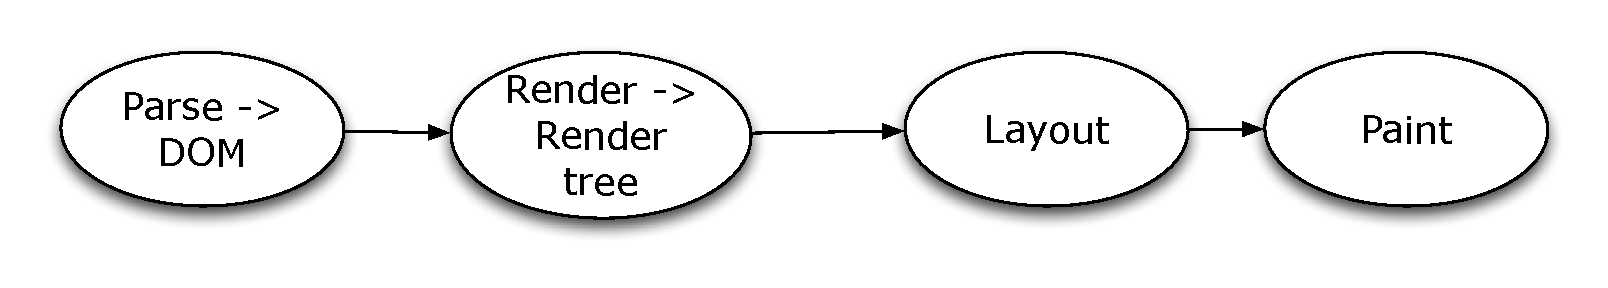
\includegraphics[width=11cm]
{rendering.eps}}
% Kommandoen \fbox tegner en ramme.
\end{center}
\caption{The rendering engine's responsibility}\label{fig:render}
\end{figure}

WebKit\cite{webkit} and Gecko\cite{gecko} are two popular rendering engines that implements the rendering process in figure \vref{fig:render}, however they do differ slightly in their internal behavior. WebKit is the engine that runs Chrome and Safari, while Gecko runs Firefox. In this section we limit the discussion to concern only these platforms, as they are built upon open source solutions and thus have available technical descriptions. The text that follows describes the process of rendering a complete HTML page. This usually happens when the client-browser requests a URL for an HTML page and the browser "refreshes" the page with the new content.

\paragraph{Parsing} 
The rendering of an HTML page starts when the networking layer is instructed to fetch a URL, say \textit{www.google.com}. Once the HTML page is fetched, the browser will immediately start fetching all external \textbf{links} that are contained inside it, from top to bottom. This could be links to CSS stylesheet pages, JavaScript pages, images, videos, etc. The rendering engine will continuously request chunks of HTML and CSS data from the networking layer, that it parses. An important feature of the HTML document's structure is that all the markup elements (tags) are nested in a hierarchical structure. Thus, when the HTML document is parsed, its tags are laid out in a tree structure.

Whenever the parser hits a script tag, it will first fetch the script if it is referencing an external file. Then, it will execute the script immediately. Unless the tag is marked "deferred" in which case the handling of the script will be postponed until the HTML parsing is done, the parser has to wait until the script is both fetched and executed. This is because the script might try to manipulate the HTML. To improve performance by avoiding the HTML parser to block while scripts are loaded, scripts can also be marked as "async" in which case the modern browser will generate a separate thread that fetches (if the script is not embedded in the HTML) and parses the script, while the main parser thread can continue and parse HTML. 
 
 The tree that is generated is called the \textbf{DOM tree}, where each tree element is named a DOM element. The DOM tree offers a programming interface (API) that can be used by JavaScript in order to manipulate the HTML. When the whole HTML page is completely parsed, the rendering engine will start executing the scripts that are marked "deferred". When these scripts are finished executing, the browser will generate a \textbf{DOMContentLoaded} event. Finally, when all the external resources are fetched and parsed, the browser will generate an event called the \textbf{load event}. The purpose of these events is that JavaScript execution can be set to execute, first once any of them is triggered.

\paragraph{Rendering}
While the DOM tree is being populated, the rendering engine will also start generating the \textbf{Render tree}. This is another tree that is a visual representation of the DOM tree, and in effect decides the style and order of how the DOM elements should be laid out. Every element in the Render tree has a reference to its DOM node, a style, and in addition they know how to layout and paint itself and its children. In effect each render element represents a visual rectangle on the screen. 

\paragraph{Layout and Painting}
In the layout process, each render element is given coordinate instructions for where on the screen it will be placed, and its size. The calculation is performed recursively from the root HTML node to the bottom.
The painting process does the actual work of painting the elements on the screen. It does so by iterating through the rendering tree and paints each component.
 
\subsection{JavaScript}
JavaScript is an interpreted programming language primarily built for manipulating Web pages. The language was developed at Netscape in 1995, during the time when Netscape and Microsoft were battling for the majority of browser users. The language itself was built in only 10 days, by Brendan Eich\cite{jsin10days}. He had instructions to develop a language that would look like Sun's Java, only simpler, interpreted and easy to integrate into Web pages, so that it would appeal to non-professional developers. Eich designed the language to follow much of the syntax from the C programming language, only simpler and with a much more dynamic memory management system. 

Despite a considerable amount of buggy features in the language and some compatibility issues between the different browsers, JavaScript quickly became a  popular language for the Web. Developers could easily create interactive behavior like changing color on a button when a mouse hovers over it, give the user feedback if the input in a textfield is wrong, etc. Much of its success was because of its simplicity; there was a low barrier to add JavaScript behavior into Web sites. Because there is no compilation process, and no "start function", only independent functions that can easily be written and ``tossed'' around in the document, unprofessional developers could quickly implement exciting and dynamic features \cite{jsHowGotHere}. On the other hand, for this reason, many professional developers would consider the language of being strictly for amateurs and not suitable for professional developers \cite{UnderstoodJs}.  Its strength was clearly for small sized applications, as browsers at the time were not able to execute large-scale JavaScript code. Also, considering that the JavaScript language at the time was very simple and limited, the development of large-scale JavaScript Web applications was simply not feasible. 
 
In an effort to improve the language features of JavaScript, and its browser incompatibilities, a standardization process of JavaScript was given to the European Computer Manufacturers Association (ECMA) in 1996. The language was actually renamed to ECMAScript, although most people still refer to it as JavaScript \cite{jshist}. Unfortunately, as the standardization was being developed, the browser inconsistencies, especially between Netscape and Internet Explorer continued to grow. Many JavaScript frameworks were built as workarounds to the inconsistencies, but most solutions weren't good enough. This led to alternative solutions for highly interactive and graphical client-side behavior such as Adobe Flash\cite{flash} or Microsoft's Silverlight\cite{silverlight}. 

An important part of JavaScript's history was with the rise of \textbf{AJAX} (Asynchronous JavaScript and XML) technologies\cite{ajax}, which gained much attention right around a century after JavaScript was first introduced. AJAX is an API that offers JavaScript functions that makes the browser asynchronously fetch data from the server without having to refresh the current Web page. Instead, the requested data would be used to alter the  page. This would result in a much more interactive user experience because the browser would neither block while waiting for the result, or re-render and paint the whole DOM tree upon successful complete. Since the introduction to AJAX, JavaScript has increasingly become a very popular language, and it has also brought the attention of professional developers. This has led to successful framework solutions like JQuery\cite{jquery} and Prototype\cite{prototype}, which simplifies the development of complex dynamic behavior and fixes browser incompatibilities, so that the Web developer doesn't have to write specialized code for each browser.

The increasing popularity of client-side application development with JavaScript has led to powerful JavaScript engines in modern browsers, making memory management and JavaScript interpretation highly effective. In September 2008, Google built the Chrome browser with its V8 JavaScript engine\cite{v8}, stating that low performance JavaScript implementations are no longer sufficient. Other browser vendors followed along, and today JavaScript performance is more superior than ever. Still, however, there are drawbacks with the language itself. Even though libraries like JQuery and Prototype simplifies the development of interactive and cross-platform Web pages, it is easy to end up with a big pile of tangled JavaScript event handlers and unstructured functions (often called spaghetti code\cite{spagetticode}). Most of the reason is that the language lacks features like classes, modules and namespaces, which makes it difficult to develop flexible and maintainable large-scale JavaScript applications. However, a lot of work has been done lately to implement quality frameworks that provide comprehensible syntactic sugaring for the language. These frameworks use some of the nice, and for many unknown concepts of the JavaScript language such as inheritance and closures to enable a highly flexible and structured development environment. All this has led to the possibilities of building large-scale JavaScript Web applications that runs primarily in the browser. Good examples are Google's Gmail\cite{mail}, and Maps\cite{maps}.

\paragraph{Node.js}\cite{node} is a Web application framework built for using JavaScript as the programming language. This is one of the first (and most popular) solutions for developing JavaScript Web applications on the server. It runs on Google's V8 JavaScript engine. A big advantage this framework has compared to other frameworks such as Rails or Spring, is that it is single-threaded and event-driven. This is a completely asynchronous programming environment that is centered around events, where clients subscribe to events and are notified when the events are triggered. This avoids the blocking scenario that might occur in regular synchronous systems. 


\subsection{Client-server Interaction Schemes}
There are multiple ways the browser can communicate with the Web server. In this thesis, we mainly adhere to two different ways. Synchronous client-initiated requests, and asynchronous client-initiated requests. These communication schemes all use HTTP, and are client-pull based. However there are other push-based alternatives such as Comet\cite{comet}, and WebSocket\cite{websocket}, where the client and server maintains an open connection, and the server can notify the client of changes.

\paragraph{Synchronous}
In a synchronous HTTP requests, the client-browser asks the server for data, in which the browser will wait for the server to respond. The request is normally trigged by the user clicking an anchor tag (hyperlink), or submits an HTML form. This would usually result in a new HTML page that is returned to the browser, in which the browser would  start a complete rendering process to build a new DOM tree, and paint it on the screen. A normal term for this is a page \textit{refresh}, or \textit{reload}.

\paragraph{Asynchronous}
In asynchronous HTTP requests, the client sends a request to the server, without the browser having to block while waiting for the result. Usually this happens with an AJAX request. When the result is received from the server, a browser event is triggered that is normally picked up by a JavaScript handler function. Typically the JavaScript handler alters the DOM tree with the new data received from the server.

One potential drawback with AJAX is that not all browsers support JavaScript. Examples are some smartphone devices or PDA devices.  Also, pages that are generated using AJAX are not automatically picked up by Web crawlers, because most Web crawlers do not access JavaScript code. This means that content generated by AJAX would normally not show up in public Web searches. However, in 2009, Google proposed a programming technique to make AJAX pages crawlable\cite{ajaxcrawl}. This is a somewhat complex technique, and can be tedious to implement in larger JavaScript applications.


\subsection{HTTP Sessions}
An HTTP-session is a semi-permanent communication dialogue that exists for two communicating entities (here, the client and the server). A session normally has a time-out value, such that when the time runs out, the session ends. The HTTP protocol is stateless in its nature, because every HTTP request is self-contained, and independent of every other request. Therefore, to be able to maintain state in an application, the client and server can incorporate a session protocol. The state information itself is data that has to be maintained between multiple pages in the application. Examples are shopping cart information in an e-commerce site, flight booking details, or authentication credentials. Imagine the user having to identify himself for each request that is sent to the server. This can be avoided if state information is persisted and being referenced in each request. 

There are a couple of ways to implement sessions:
\begin{itemize}
\item{} An object that is kept on the server . This object can be referenced in the client's cookie, or in the URL, if cookies are not supported. 
\item{} In the messages sent between the client and server, for example by populating the cookies, or keeping the data in the HTTP request and response body, or in the URLs. Clearly the size of the session data is very limited in this case.
\item{} In the browser's own storage system, thus maintaining sessions only on the client.
\end {itemize}

\subsection{Representational State Transfer}
Modern Web applications often follow a design pattern named Representational State Transfer, or simply REST \cite{armando2012}. This pattern states that all HTTP URL's must reference a particular resource on the backend, by using one of the HTTP request methods Get, Post, Put, or Delete (HTTP also supports additional request methods, but these are the most commonly used). This way, every URL offered by the Web application are self-contained in that it contains all the necessary information needed to satisfy a request. Resources are uniquely identified by a URI, and manipulated through the HTTP method interface. Applications that follow this pattern are named RESTful applications. A common use case for RESTful applications is to offer the self-contained URL's publicly as an API to clients other then just the application's own front-end, like other third party applications that wishes to use the applications REST services. Further, the REST pattern states that each REST request is stateless, hence adhering to the nature of HTTP which is stateless. That means, REST requests should not depend on an ongoing session in order to generate proper results.

\subsection{JSON}
JSON\cite{json} (JavaScript Object Notation) is a text based data format that is based on a subset of the JavaScript programming language. It is easy for both humans to read, and machines to parse, and has a similar syntax to many of the programming languages based on the C family of languages. The data structure fits well as a transmission format in Web applications, because it is both simple and light weight, easy to modify and is supported by many programming languages. The format itself is very simple, and the datatypes offered are limited to numbers, strings, arrays, booleans, and objects (being key-value pairs of the types just defined). An example of a JSON object representing a guitarist is showed below:
	\begin{lstlisting}
	{
		"username": "Paul ShredKing",
		"age":21,
		"country": "Norway",
		"guitars": 
		[
			"Gibson Les Paul",
			"Fender Stratocaster"
		]
	}
	\end{lstlisting}
The closest alternative to JSON is XML\cite{xml}, which is another transmission format often used on the Web, and especially with REST communication. However, its syntax is a bit more verbose, and requires more processing to manage because of its complex markup tags and syntax rules. On the other hand XML lets one add more restrictions to the data then with JSON.

\subsection{Business Logic and View Logic}
In Web applications, one often separates two very different programming concerns; the business logic and the view logic. The business logic (also called domain logic) typically represents:
\begin{enumerate}
\item{} The application's \textbf{domain}, often called business objects. They describe the application's core entities. Classical examples are Account, User, Purchase, Loan etc
\item{} The operations that can be performed on the business objects
\item{} Interactions between the business objects, and business rules that state the values that business objects are allowed to have
\end{enumerate}
The view logic (often called presentation logic) describes how the domain is visualized in the user interface. The view logic implements dynamic user interface behavior. It is often generated on the server, and depends on the application's current state. Typical Web 2.0 applications contain complex view logic.

Separation of business logic and view logic is considered best practice\cite{sepbiz} in order to let one concern change independently of the other, and to enhance a coherent codebase where separate concerns does not directly depend on each other\cite{bestprac}.



\subsection{HTML Template Rendering}
In dynamic Web pages, when an HTTP request comes in for a particular HTML page, the server has to prepare the HTML page with proper content based on the data received in the request. One way to generate dynamic HTML (that is, perform view logic) is to generate the HTML directly in code as Strings, and send the result back to the client. However this approach is messy, difficult to maintain, and the developer has to know the programming language that is creating the HTML strings. In other words, not a preferable solution for Web designers who only knows HTML. The preferable approach is a process called HTML template rendering. With HTML template rendering, a template system is organized as a set of \textbf{template files} (often called \textbf{views}), some domain and state data, and a rendering engine. The template files are implemented in a special template language. This is basically just HTML with additional syntax that refers to and can operate on data variables in the Web application. The operations supported are usually limited to simple loops and conditional expressions, just enough to facilitate the injection of dynamic data without confusing front-end designers. To generate a page, the rendering engine takes as input one or more template files, the data needed to populate the templates, and produces as output an HTML page. The necessary data is often fetched from the database or exists already in the server's memory. The resulting HTML page is sent back to the client. 

Recent JavaScript technologies have also enabled HTML rendering to happen in the client. The process is very similar. HTML template files can be sent to the client, which are ignored by the browser so the browser won't automatically paint them on the screen. Special JavaScript rendering engines that does the same job as the server-side rendering engine recently described can be accessed by JavaScript code in the browser. When some HTML template is to be rendered, the JavaScript rendering engine is called with an HTML template and a data object as input, and it returns an HTML page populated with the data content. The resulting HTML is typically appended to the DOM, or swapped with existing DOM elements. 

\subsection{Databases}
Databases, and especially relational databases have since the beginning of Web application history been the most popular form of storing persistent data\cite{armando2012}. Other alternatives have also been used such as flat-file storage (where the content is stored as plain text or binary data) or XML- or object databases. Much of the reason for the success of relational databases however, is that it provides \textbf{durability}, which in the context of data persistency means that once the data is stored, it is guaranteed to exist even if machines holding the data crashes. Also, a reason for the relational database's popularity is that it stores information in a structured format, which often fits the structured data formats that are manipulated by the Web applications. However, other types of databases that differs from the traditional SQL format has recently entered the marked. These are commonly referred to as NoSQL databases.

\subsubsection{ACID}
ACID is a popular term in the context of databases. It is a set of properties that guarantees reliability when it comes to transaction management. Database management systems often state that ACID guarantees are provided in their system, in order to promise a reliable database solution. Each property is defined below:
\paragraph{Atomicity} guarantees that either all the commands in a transaction completes, or non do.
\paragraph{Consistency} guarantees that all the data will always be in a consistent state according to pre-defined rules. A transaction brings the system to a new consistent state.
\paragraph{Isolation} guarantees that parallel transaction executions are always processed as if they happen serially, i.e no interference of any two parallel transactions. 
\paragraph{Durability} guarantees that committed transactions are safe, and lasts even during system errors or crashes. 

ACID guarantees are often provided by relational database management systems (RDBMS). However, NoSQL databases tend to have more relaxed relations to the principles, in favor for speed and simple replication abilities. 

\subsubsection{CRUD operations}
In Web application terminology, one often use the word CRUD to refer to the four essential  database operations; \textit{Create}, \textit{Read}, \textit{Update} and \textit{Delete}. These are the main operations performed by the Web application, on the data that needs to be persisted. When a CRUD operation is executed, it is the application's responsibility to convert the data into a format that fits the database's technology, and vice-versa. This process is called \textbf{marshalling}, or serializing. One example is when the application is to save a new object in the database. In this case, a \textit{Create} operation will be performed where the application will transform the object from whatever programming language syntax the object is currently described in, into a structure that fits the given database's syntax. The application will send this transformed (marshalled) object to the database, which is now able to parse the object and save it to its storage structure.   

\subsubsection{Relational databases}
Relational database management systems is a storage system based on a formalism known as the relational model. The formalism is based on structure and relationships, where the data entities are stored into \textbf{tables} that contain a set of \textbf{attributes} that describe the table. The tables can be related to each other to form groupings. RDBMS's stores a collection of tables, where each data entity is represented as a \textbf{row} in a specific table, and each column in a row represents an attribute for that entity. The most popular form of manipulating data in a RDBMS is SQL (Structured Query Language)\cite{sql}. This is a query language used to insert and manipulate data in a relational database. There are popular dialects of the language, generated by database vendors such as Oracle's SQL\cite{oracle}, Microsoft's MS SQL\cite{mssql}, MySQL\cite{mysql} and the open source PostgreSQL\cite{postgresql}.

\subsubsection{NoSQL}
NoSQL is a broad class of various database management systems who all have in common that they don't share the relational structure from normal SQL databases. The reason for its existence starts with the rise of Web 2.0 applications, when developers saw the need for simplifying replication of data, higher availability, and a new way to manipulate data that can avoid the need to perform tedious mappings between SQL strings and objects in any given programming language\cite{tedorm}. The main potential for NoSQL databases is to perform operations on massive amounts of data that is not structured or connected in complex relationships. Very often this applies to Web 2.0 applications, because much of the information in such applications can be gathered in coherent entities, thus avoiding the need for complex relationships and tedious operations to join them together. A typical example is users that has arrays of blog posts, and blog posts has arrays of comments, in which case all these fields are nested inside the user abstraction.

What's typical with NoSQL is that they are often customized to solve a particular type of application's persistency need. Therefore, there are many different classifications of NoSQL databases, which vary in the way they structure the data. An overview of the some commonly used NoSQL categories is summaries in the following list:
\begin{description}
  \item[Key/value store] \hfill \\
	Is a simple database store where data is identified by a key, and the data itself can be any datatypes usually supported by the implementing programming language. The structure is schema-less, meaning it doesn't provide complex structures with foreign key constraints. It is also highly efficient as the database is often implemented as a HashMap. One popular example is Redis\cite{redis}. This is an extremely fast key-value store that favors speed over durability. It also provides simple replication support, making it easy to distribute the database over multiple machines. Much of the reason for Redis' extremely high speed is because the data is typically being kept in memory, and only written to the database as a snapshot every once in a while. Other popular key/value stores are Riak\cite{riak} which favors scalability and fault tolerance, and Voldermort\cite{voldermort}, which favors simple distribution (data is automatically replicated). 
	
  \item[Document-oriented databases] \hfill \\
  Is a datastore that is based on documents that contain unstructured content. Documents are often separated into unstructured collections (can be viewed upon as SQL-tables), where unstructured here means that content in the same collection can have different structure. However there is some variation in the way the different database implementations choose to define the formats of the documents, but it can be assumed that each document encapsulates some logically associated data in a predefined format. An interesting property with these databases is that performance is often not the main goal, but rather programming satisfaction. As many of these are implemented in JavaScript and offers querying semantics and data structures based on JavaScript objects, it is really easy and flexible to perform database operations on them. Examples include CouchDB\cite{couch} and MongoDB\cite{mongo}.
  
  \item[Column-oriented databases] \hfill \\
  Is a database system where data is organized as columns, as opposed to row-oriented databases such as SQL based databases. In this scenario, every value that would usually be in a row gets its own instance in a column together with its belonging identifier (Id). As such, it is very efficient to perform range queries over a big amount of column data. Examples are Cassandra\cite{cassandra} and Google Big Table \cite{bigtable} (although these are not pure column-oriented, but rather a hybrid). 
\end{description}

\section{Summary}
We started this chapter by looking at how the World-Wide-Web began in the late 80's. In the beginning, Web sites were primarily a collection of static pages, but gradually turned into more dynamic pages where the content changes depending on attributes provided by the client. After this we saw that some of the technologies that are found on the Web today are outcomes of the browser wars that started in the mid-90's. This especially concerns the JavaScript programming language, which has resulted in many browser incompatibilities and a somewhat misunderstanding and unawareness of JavaScript's core language features and capabilities. However, major browser vendors, and Google especially, has acknowledged the advantage of having a unified language for the Web, something that has brought a lot of attention and improvements to the JavaScript programming language and its related technologies. This has now made JavaScript become a highly popular language for the Web, and developers have started building large-scale dynamic Web applications purely in JavaScript.

In the second part of this chapter, we looked into popular technologies that are commonly found in modern Web applications. Examples included AJAX, which offers an asynchronous client-server communication scheme, REST, which is a design pattern that states that Web resources should be manipulated exclusively through methods specified in the HTTP protocol (get, put, post, or delete), and NoSQL databases, which are databases that doesn't abide to the relational model, but instead specializes in speed and scalability through replication. We also looked at a specific type of modern Web applications, namely Web 2.0, which we saw were interactive Web apps with responsive and rich user interfaces, and social networking features.  

   
